\section{準備}
本章では,本論において核となる技術内容・特徴およびそのメカニズムについて説明する.
\subsection{DNS プロトコル}
\label{sec:dns-protocol}
DNS(Domain Name System)は,インターネットに接続された無数のコンピュータを一意に識別するためのIPアドレスを,人が認識しやすいドメイン名に変換するシステムである.
元来,インターネット上でのホストの識別にはIPアドレスが使用されてきた.
しかし,32bitの名前空間で10進数表記のIPv4(E.g. ``192.168.0.1"),もしくは,128bitの名前空間で16進数表記のIPv6(E.g. ``2001:200:16a:8::230")は,人にとって認識しにくいものである.
そのため,自然言語のようにアルファベットや数字で表記する方法が取られ,当初はその対応表であるhosts.txtが中央集権的に管理されていたが,やがてホスト数の増大に伴い管理が困難になっていき,提案されたのが対応表を分散的に管理するDNSである.

DNSのシステムアーキテクチャは,クライアント・サーバ構成で成り立っている.
一般に,クライアントがドメインを問い合わせた場合,サーバはドメインに対応づけているIPアドレスを応答することで,クライアントはドメインに対応づけられたIPアドレスを解決することができる.
ドメインからIPアドレスの解決は正引きと呼ばれ,IPアドレスからドメインの解決を逆引きと呼ぶ.

ドメインは,数字とアルファベットおよびハイフン(``-")の文字列で表記され,最大長は63オクテットと定義されている.
また,ドメインはルートを頂点とする階層構造をとり,各階層にはドメインを管理する主体が存在し,管理主体を委譲することによって分散的にデータベースを管理する仕組みを取っている.

\begin{figure}[h]
 \centering
 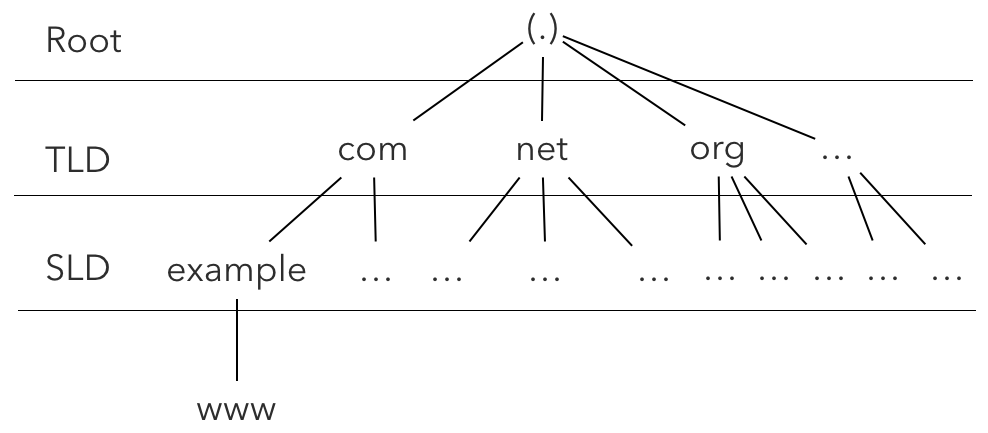
\includegraphics[width=12.0cm]{figure/dns-architecture.png}
 \caption{ドメインにおける名前空間}
 \label{fig:dns-architecture}
\end{figure}

ドメイン名は,ドメインに相当するラベルをドット区切りで表され,最大長は255オクテットである.
ドメイン名は右から順に階層序列が表現され,ドットで表現されるルートは一般には省略される.
最も右に位置づくラベルがTLD(Top Level Domain)であり,そのTLDからn番目(n $\mid$ n $\in$ $\mathbb{N}$)のラベルが第 n レベルドメインである.

TLDを大別すると,``.com"や``.net"をはじめとした特定分野別のgTLD(global Top Level Domain),``.jp"や``.ch"のような国ごとに割り当てられているccTLD(Co\\untry Code Top Level Domain)の二つに分けられる.
%TLDごとに登録するプロセスや必要書類,金額は異なり,上いの

%\subsubsection{ノードの種類}
DNSは,機能に応じて3つに分類することができる.

%\subsubsection{リソースレコード}
DNSの仕組みにおいて,ドメイン名に関連づけられた情報は,IPアドレス以外にも様々なものがあり,それらはリソースレコード(Resorce Record, RR)と呼ばれる.
DNSの仕組みによって,権威サーバが提供できる情報はドメイン名とIPアドレスの対応情報だけではない.
最も一般的なレコードは,Aレコードであり,FQDNをIPv4アドレスにマッピングする.
権威は,サブドメインへ委譲することが可能である.この機能は,NSレコードによって実現される.

\subsection{DNS Exfiltration}
\label{sec:dns-exfiltration}
DNSを利用して情報を外部に転送するには,初めにデータの宛先となるドメイン(E.g. exfil.com)を作成することになる.
転送する際のキャリアとなるDNSクエリのラベルには,使用できる文字列は数字・アルファベット・ハイフン(``-")である必要があるため,一般にBase32・64を用いて転送したい情報をエンコーディングすることでこの制約条件を満たす.
用意できたQNAME(E.g. arbitrary-string.exfil.com)について,例えばAのリソースレコードをクエリすると,サブドメインの存在の有無に関わらず,宛先となるドメイン(exfil.com)に任意の情報を転送することができるという具合である.
以下\ref{fig:dns-exfiltration}に,DNS Exfiltrationのメカニズムについて図解する.

\begin{figure}[h]
 \centering
 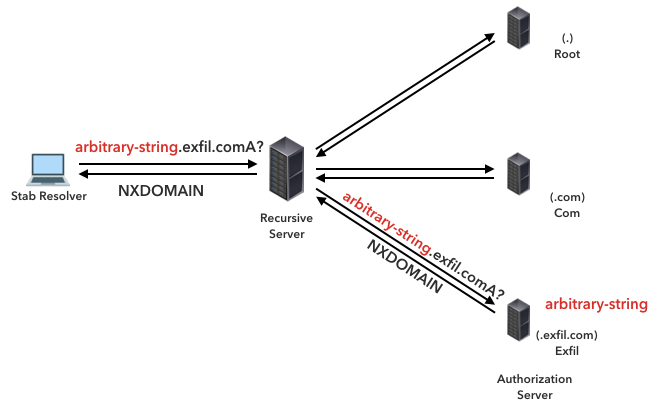
\includegraphics[width=12.0cm]{figure/dns-exfiltration.png}
 \caption{arbitrary-stringという任意の文字列が,DNSクエリのラベル部を用いて,事前に用意した権威サーバ(exfil.com)に転送される様子.}
 \label{fig:dns-exfiltration}
\end{figure}

また,管理する権威サーバのドメインに適当なホスト名(E.g. www)を作成し,そのホスト名のリソースレコード(E.g. TXT)に情報を付与していた場合には,そのホストへの問い合わせを通じて逆方向,すなわち権威サーバから任意の情報を転送することができる.
DNSのリソースレコードを転送キャリアとする流入通信のメカニズムを図解した様子が,\ref{fig:dns-tunneling}である.

\begin{figure}[h]
 \centering
 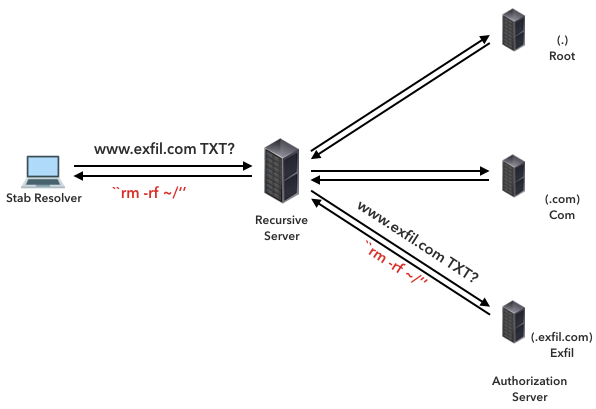
\includegraphics[width=10.0cm]{figure/dns-tunneling.png}
 \caption{事前にTXTレコードに登録された情報を問い合わせることで,権威サーバからの命令情報を取得している様子.}
 \label{fig:dns-tunneling}
\end{figure}

このようなDNSを用いて双方向な通信手法がDNS Tunnelingである.
%1998年4月,DNS Tunnelingの手法は,NmapのBugtraqメーリングリストにて初めて公になったとされている\cite{bugtraq}.

\subsection{DNS Infiltration}

%\subsubsection{DNS Tunneling 特徴}
%%\subsubsection{その他課題}
%%\subsection{秘匿通信}
%%秘匿通信(英Covert Channel)とは,
%%情報転送を実現するにあたり,データの転送を本来の設計としていないプロトコルにそのデータを注入する手法である.
%%\subsubsection{ステガノグラフィ}
%%\subsubsection{代替プロトコル}
%\subsection{分散ハッシュテーブル}
%\subsubsection{アルゴリズム}
%\subsubsection{暗号学的ハッシュ関数}
%\subsection{P2P}
%\subsubsection{アーキテクチャ}
